

%%%%%%%%%%%%%%%%%%%%%%%%%%
%%%%%%%% Comment %%%%%%%%%
%%%%%%%%%%%%%%%%%%%%%%%%%%
\begin{comment}
General about the platform. Tjek the initial analysis.
Moodle uses innodb and mysql (in our case atleast) 
PHP.
\end{comment}
%%%%%%%%%%%%%%%%%%%%%%%%%%
%%%%%%%%%%%%%%%%%%%%%%%%%%

\section{Constraints}
\label{sub:constraints}
Moodle is written in the programming language PHP~\cite{moodleabout} and uses an SQL database.
This restricts us to write \system{} in PHP as the server side scripting language.
Since \moodle{} uses an SQL database system we choose to restrict ourselves to use that as well, to avoid adding unnecessary dependencies to third party systems.


\section{Courses}
\label{sub:courses}
Courses is a fundamental concept in Moodle, since Moodle is a course management system.
Courses can use activity modules, which are described further in \secref{sub:plugins}, and are often split into sections depending on the selected course format.
One example of a course format is the weekly format which splits the course into a section for each week~\cite{moodlecourseformat}.
Every course in Moodle is part of a course category~\cite{moodlecoursecategories}. 
Course categories can be hidden such that students and lectures are not able to see the courses in these categories on the Moodle page, though administrators are always able to find courses even if they are hidden.


\section{Groups}
\label{sec:groups}
Moodle has a built-in concept of groups and groupings. 
Groups can contain users and groupings can contain groups. 
The database scheme of groups and grouping can be seen on \figref{fig:moodlegroupsandgroupings}.

\begin{figure}
	\centering
		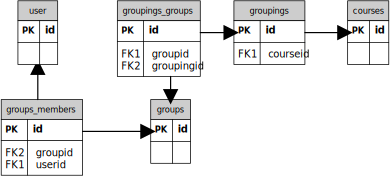
\includegraphics[width=\textwidth]{images/moodlegroups}
	\morscaption{The database scheme for groups and groupings. Data fields that are neither part of a primary key nor foreign key are omitted for clarity~\cite{moodleerdiagram}}
	\label{fig:moodlegroupsandgroupings}
\end{figure}

This structure supports that users can be in groups and that more groups can be grouped together in one grouping. 
One group can be a part of several groupings and a user can be a member of several groups. 
The foreign key from groups to course and the foreign key from grouping to course indicates a tight connection between groups and courses.
In fact every group and grouping must refer to a course, to which the group or grouping is said to belong.

\section{Plugins}
\label{sub:plugins}
As mentioned in \secref{sub:lms} the ``M'' in Moodle stands for Modular. 
Moodle currently supports 34 types of plugins~\cite{plugin}.
The four most common plugins are explained below:


%http://docs.moodle.org/dev/Plugins


\paragraph{Blocks}
\label{subsec:blocks}
%http://docs.moodle.org/dev/Blocks
Moodle uses the term block to refer to a box that can contain a wide spectrum of information and functionality.
A block can as per default be placed in the left or right side of a page. 
Pages can allow placement of blocks in the center of a page.
The navigation block~\cite{navigationblock} is a very common block, which as per default is displayed on all pages. 
It contain links such as My Profile and My Courses. 
Blocks are not limited to navigational purposes, but can also display data from the database.

Each block has settings regulating which pages it can be displayed on. %Blocks can be places in number of different regions if the theme allows it. 

%Blocks are intended to display information or be used as a small tool.
%``Small information-displays or tools that can be moved around pages''
%Hvornår er det godt at lave en block
%http://phpdocs.moodle.org/HEAD/core/lib/moodle_page.html
%http://phpdocs.moodle.org/HEAD/moodlecore/moodle_page.html



\paragraph{Activity modules}
\label{par:activitymodules}
%http://docs.moodle.org/dev/Activity_modules
%http://docs.moodle.org/22/en/Activity_modules
%http://docs.moodle.org/22/en/Activity_modules_administration
``An activity is a general name for a group of features in a Moodle course.''~\cite{activity} 
Activity modules are the main way to create new features in a course, and a new feature is called an activity. 
It is common that a course page contains an activity block~\cite{activityblock}, that contains available activities for the course. 

Activity modules often contain a new page where an activity is available. 
An example of this is a forum. 
On the course page there is a link -- when it is pressed the forum page is displayed. 
An activity is saved with the course, which means that several individual forums can exist on different courses.

Activity modules are intended to be used when making a feature that interact with several users in the context of a course.  
%show table; mdl_modules -> mdl_activities 
%hvornår skal man lave et am

%``Activity modules are the most important type of plugins. They provide activities in courses. For example: Forum, Quiz and Assignment.''
\paragraph{Admin tools}
\label{par:admintool}
%http://docs.moodle.org/dev/Admin_tools
Admin tools are, as the name implies, tools used for administrative purposes. 
The Moodle Developer Documentation defines the functionality of an admin tool as the following: 
``Provides utility scripts useful for admins to examine and modify a Moodle site''.~\cite{plugin} 
The only users that can access the admin tools are administrators. 
These are made available through the Site administration menu point in the Settings block~\cite{moodleadmintools}.

\paragraph{Local plugins}
\label{par:localplugin}
%http://docs.moodle.org/dev/Local_plugins
Local plugin is the most general type of plugins. 
If the wanted feature does not fit the other types of plugins, it is recommended to use the local plugin. 
An example of this is communication with an external system or for extending the navigation block. 

%Local plugins are intended to be used when making new functionality in Moodle. 


\section{Framework}
Moodle includes various APIs~\cite{moodlecoreapis}, which aid the developer in the process of creating an extension. Some of the APIs are:

\begin{itemize}
	\item Data Manipulation Language (DML) API~\cite{moodledml} for all persistent data access and is described further in \secref{sec:moodleoplatformdbml}.
	\item Form API~\cite{moodleformapi} for rendering HTML form objects and handle the validation of the data sent through the form. 
	\item Output API~\cite{moodleoutputapi} for general HTML rendering.
	\item Page API~\cite{moodlepageapi} for setup of a standalone page including methods for adding JavaScript and configuring display options. 
	\item Access API~\cite{moodleaccessapi} for controlling access levels of users throughout the Moodle installation. 
	\item Unit test API~\cite{moodleunittestapi} for testing components in Moodle.
\end{itemize}
Moodle APIs are used in different ways. 
The DML API, Page API, and Output API are used through global variables, whilst the others are used through class extensions. 
In~\coderef{moodleapiusage} usage of Page API and Form API is shown.
\begin{lstlisting}[style=phpCode, caption=\myCaption{Example of the Page API and Form API in Moodle}, label=moodleapiusage]
global $PAGE;
$PAGE->set_context($somecontext);

class some_form extends moodleform {
	...
}
\end{lstlisting}

\begin{comment}
$
\end{comment}


\subsection{Database Access Layer}
\label{sec:moodleoplatformdbml}
To access and manipulate data in Moodle the DML API is used.  
The API is accessed through a global variable named \vari{DB}. 
It has several methods for updating, inserting, deleting, and selecting. 
%The basic method for select, insert, and update, namely get\_record, update\_record, and insert\_record, take or retrieves an object of type stdClass.
The basic methods for selecting and inserting are \fu{get\_record} and \fu{insert\_record}.
These either accept an argument of type \cl{StdClass} or return one generated from data in the database.
\cl{StdClass} is a standard PHP class which is empty, and allows for arbitrary addition of properties at runtime like any other PHP object.

This gives a unified procedure for data manipulation. 
A simple update procedure is seen in \coderef{moodlecodeupdate}.
For simple operations it is not necessary to write any SQL queries, but for more complex queries, such as queries using joins, SQL statements must be written directly.
\begin{lstlisting}[style=phpCode, caption=\myCaption{Example of how to change the name of a user}, label=moodlecodeupdate]
function change_name($id, $new_name){
	global $DB;
	$user = $DB->get_record('user', array('id'=>$id));
	$user->name = $new_name;
	$DB->update_record('user', $user);
}
\end{lstlisting}


\subsection{Context System}
\label{sub:contextsystem}
The context system in Moodle is used to set the context of a given page to determine the capabilities of the user, who is currently logged in, and which blocks and activity modules to present~\cite{moodlerolesandmodules}.
 
When a user is logged in to a Moodle system he can have various roles in various contexts. 
One user may be a student in one course and a teacher in others. 
The context system is structured hierarchically.
%Moodle uses a hierarchical context system to manage roles of users and their capabilities. 
%Capabilities are described further in \secref{sub:capabilities}. 
The hierarchical layout of the context system can be seen in \figref{fig:moodlecontexts}~\cite{moodlefilemoodlecontext}.
The highest level of context is the system context, which all other contexts inherit from.
 
 \begin{figure}
	 \centering
		 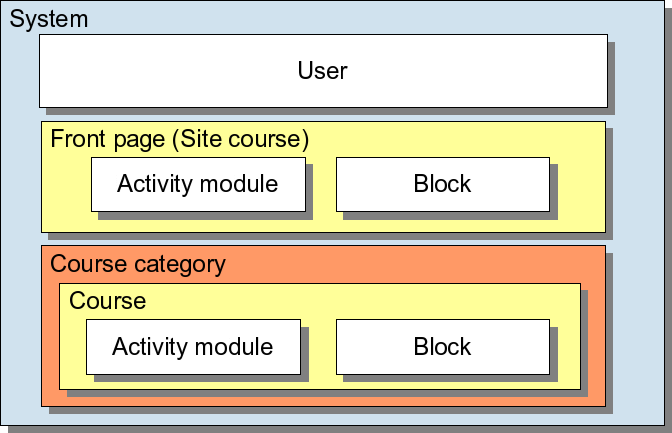
\includegraphics[width=\textwidth]{images/moodle-contexts.png}
	 \morscaption{The hierarchical context structure of Moodle. Picture source: \cite{moodlefilemoodlecontext}}
	 \label{fig:moodlecontexts}
 \end{figure}


Every webpage in Moodle must set the page context. 
An example of how to set the context can be seen in \coderef{courseviewcontextsnippet} from \moodlefile{/course/view.php}, which loads the default page of a Moodle course.

\begin{lstlisting}[style=phpCode, caption=\myCaption{Code snippet from \moodlefile{/course/view.php} showing how the context of a course is set}, label=courseviewcontextsnippet]
...
if (!$context = get_context_instance(CONTEXT_COURSE, $course->id))
{
	print_error('nocontext');
}
...
\end{lstlisting}
The function \fu{get\_context\_instance} requires a context level and in this case also a course id. 
The context level used in the function call is a constant telling which context level that needs to be loaded. 
This is a numeric value. 
In this example an error is outputted if the context fails to load. 
This happens if the context level provided is illegal or in this instance if the course id in invalid.
%To determine if a user has the capability to do a certain action the function \fu{has\_capability} is used~\cite{moodlerolesandmodules}.
%It requires a string specifying which capability and the context for the current page. 
It is required to set the context for each page. 
In some pages Moodle sets the context itself~\cite{moodlepageapi}. 

%Beside being responsible for capabilities, contexts are used to determine the presented blocks on a page.
If a user adds an instance of a block and the context is set to the system context, the block instance will be shown on all course pages.
If the context is set to the course context the block instance will only be presented on the page of the course.

\begin{comment}
\subsection{Capabilities}
\label{sub:capabilities}
Moodle integrates a capability system to manage permissions throughout the site \cite{moodlerolesandmodules}. 
Every capability is connected to the system context, which is global for the entire site. 
Capabilities can be changed in inherited contexts. 
For example a user who does not have a permission in the system context to create courses can have the permission to do so in a certain course category. 

Creating new capabilities is possible when creating a new plugin. 
To check capabilities the function \fu{has\_capability}, which takes a capability, given as a string, a context instance and extra parameters depending on the capability and the context. 

\end{comment}